\chapter{Introducci'on}

\section{Los problemas}

Supongamos que estamos a cargo de la distribuci'on de la edici'on f'isica de un importante diario en una gran ciudad, para clientes suscriptos. Las entregas se hacen al domicilio de cada cliente, utilizando camiones de reparto, como el que se muestra en la \autoref{fig:boston}. Estos camiones circulan por la ciudad, recorriendo, uno por uno, los domicilios a los que se debe hacer una entrega.

\begin{wrapfigure}{r}{0cm}
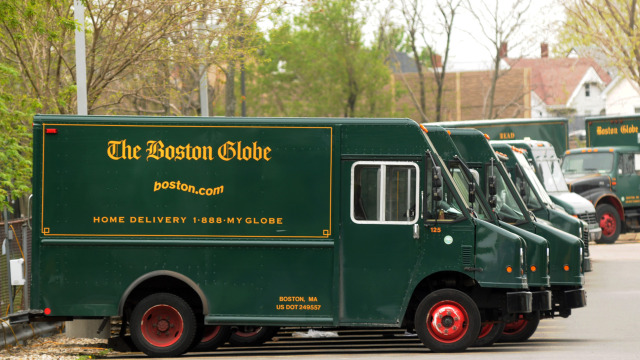
\includegraphics[scale=1.4]{img/boston.jpg}
\caption{Cami'on de reparto del diario \textit{The Boston Globe}.}
\label{fig:boston}
\end{wrapfigure}

Durante el procedimiento de reparto usual, un cami'on se detiene en la puerta de un domicilio y el conductor desciende del mismo, retira tantos diarios como haya que entregar all'i, y hace entrega de los mismos. Luego, vuelve a subirse al cami'on, y conduce hacia la puerta del siguiente domicilio.

Una alternativa a esto es un sistema de reparto en el que un cami'on no se detiene en la puerta de cada domicilio, sino en las esquinas de las calles de los clientes. Al detenerse en una esquina, el conductor desciende del cami'on, y realiza las entregas a todos los clientes que est'an sobre cada una de las cuadras incidentes a esa esquina (que suelen ser 4), a pi'e. Este sistema reduce el recorrido realizado por el cami'on, y lo compensa con recorrido a pi'e. Por lo tanto, es especialmente conveniente cuando hay una alta densidad de tr'ansito vehicular. Tambi'en es potencialmente mejor que el sistema tradicional en zonas donde hay una alta concentraci'on de clientes, a'un si hay poco tr'ansito, porque permite  realizar varias entregas, haciendo una 'unica descarga de diarios del cami'on. Notar que este sistema puede ser utilizado en otros contextos que involucren el reparto de productos, como por ejemplo la distribuci'on de encomiendas y paquetes, que realizan empresas como FedEx o UPS.

Como en toda empresa, queremos optimizar costos. En particular, queremos minimizar el recorrido que hace un cami'on, para realizar todas sus entregas. Como un primer paso en el estudio de este problema, nos vamos a concentrar en el reparto que debe realizar un 'unico cami'on. El problema que queremos resolver toma un conjunto de domicilios en los que debemos entregar ejemplares del diario, busca calcular un camino que le permita realizar todas las entregas a un cami'on (utilizando el sistema de reparto de detenciones en las esquinas), que recorra la m'inima cantidad de cuadras posible.

Podemos modelar este problema con un grafo simple y no dirigido $G$, que representa la ciudad, y un subconjunto $X$ de aristas de $G$, que representa aquellas cuadras en las que est'an ubicados los clientes. A cada arista $e \in X$ la llamaremos \textit{cliente}. Si bien podr'ia ocurrir que haya varios clientes en una misma cuadra, en este trabajo s'olo nos importa la existencia o no de clientes, y no la cantidad, en una cuadra. El problema \problem{STAR ROUTING} (abreviado \problem{SR}) consiste en encontrar un camino de $G$, tal que cada cliente tiene alguno de sus extremos en el camino, de longitud m'inima. Esto es, el camino pasa, en alg'un momento, por alguno de los cruces adyacentes a la cuadra de cada uno de los domicilios. La \autoref{fig:introduccion_1} muestra tres soluciones factibles distintas para una instancia de \problem{SR}. En ese caso, el grafo de entrada es una grilla. Esta clase de instancias es de especial inter'es, pues permite modelar adecuadamente la topolog'ia de una ciudad.

\begin{figure}[h]
	\begin{center}
		\input{img/introduccion_1.pdf_tex}
	\end{center}		
	\caption{Soluciones factibles de \problem{SR}. (a) y (b) son 'optimas; (c) no es 'optima. Las aristas en rojo son clientes, y las flechas violetas indican la soluci'on.}
	\label{fig:introduccion_1}
\end{figure}

Si una soluci'on factible visita uno de los extremos de un cliente $e$, el cami'on de entrega podr'a, si as'i lo desea, detenerse en ese punto y realizar la entrega de productos a ese (y posiblemente otros) cliente. Sin embargo, una soluci'on de \problem{SR} no establece en qu'e esquinas debe detenerse el cami'on para realizar todas las entregas. Lo 'unico que nos garantiza, es que existe alguna forma de elegir las detenciones, que permita realizar todas las entregas. En particular, podr'iamos detenernos en cada esquina del camino, y entregar a todos los clientes restantes. Esta selecci'on de paradas podr'ia obligarnos a detener m'as veces de lo necesario, incrementando el tiempo total que insume el reparto, adem'as de aumentar el desgaste del cami'on, producto de las reiteradas puestas en marcha del mismo.

Esto motiva un problema asociado a \problem{SR}, que llamamos \problem{STOPS SELECTION} (abreviado \problem{SS}). Este problema toma una instancia de \problem{SR} y una soluci'on factible para la misma, encontrar un subconjunto de v'ertices del camino, tal que todo cliente tiene un extremo en el conjunto, de cardinal m'inimo. La \autoref{fig:introduccion_2} muestra tres soluciones factibles de \problem{SS} para la instancia de \problem{SR} de la \autoref{fig:introduccion_1}-(a).\\

\begin{figure}[h]
	\begin{center}
		\input{img/introduccion_2.pdf_tex}
	\end{center}		
	\caption{Soluciones factibles de \problem{SS}. (a) y (b) son 'optimas; (c) no es 'optima. Las circunferencias verdes indican la soluci'on.}
	\label{fig:introduccion_2}
\end{figure}

Los problemas \problem{SR} y \problem{SS} son el tema de estudio de este trabajo, aunque, como adelanta el t'itulo de la tesis, \problem{SR} es el objeto de estudio principal de la tesis, y es profundamente m'as complejo que \problem{SS}.

\section{Definiciones preliminares y notaci'on}

\subsection{M'etricas}

Sea $X$ un conjunto. Se dice que una funci'on $d: X \times X \to \mathbb{R}$ es una \textit{m'etrica} o \textit{distancia}, si para todo $a, b, c \in X$ cumple:

\begin{enumerate}
\item $d(a, b) \geq 0$ (no negatividad)
\item $d(a, b) = d(b, a)$ (simetr'ia)
\item $d(a, b) \leq d(a, c) + d(c, b)$ (desigualdad triangular)
\item $d(a, b) = 0$ si y s'olo si $a = b$.
\end{enumerate}

Sobre el plano eucl'ideo $\mathbb{R}^2$ se definen varias m'etricas frecuentemente utilizadas, dos de las cuales son la \textit{distancia Manhattan} y la \textit{distancia eucl'idea}. Si $p = (p_1, p_2), q = (q_1, q_2)$, la distancia Manhattan entre $p$ y $q$ es $d_1(p, q) := |p_1 - q_1| + |p_2 - q_2|$, y la distancia eucl'idea entre $p$ y $q$ es $d_2(p, q) := \sqrt{(p_1 - q_1)^2 + (p_2 - q_2)^2}$.

\subsection{Teor'ia de grafos}

Revisamos los conceptos fundamentales de teor'ia de grafos que usaremos a lo largo de la tesis. Un tratamiento extensivo sobre teor'ia de grafos b'asica puede encontrarse en \cite{Gr05}.

\subsubsection*{Grafos, adyacencias y grados}

Un \textit{grafo simple y no dirigido} es una tupla $G = (V, E)$, tal que $V$ es un conjunto finito de elementos llamados \textit{v'ertices}, y $E \subseteq \{\{u, v\}: u, v \in V, u \neq v\}$ es un conjunto de pares no ordenados de v'ertices, llamados \textit{aristas}. Es \textit{no dirigido} porque las aristas no tienen direcci'on, y \textit{simple} porque no hay m'ultiples aristas entre un mismo par de v'ertices, ni aristas con sus dos extremos en el mismo v'ertice. Para abreviar, diremos simplemente \textit{grafo}. En ocasiones, llamamos $V(G)$ y $E(G)$ a los conjuntos de v'ertices y aristas de $G$, respectivamente. Dada una arista $\{u, v\}$, sus \textit{extremos} son los v'ertices $u$ y $v$ que la componen.

En un grafo $G = (V, E)$, dos v'ertices $u, v \in V$ se dicen \textit{adyacentes} si $\{u, v\} \in E$. La \textit{vecindad} de un v'ertice $u \in V$ es el conjunto $N(u) = \{v \in V: u \text{ y } v \text{ son adyacentes}\}$. El \textit{grado} de un v'ertice $u \in V$ es $d(u) = |N(u)|$. Los grados de los v'ertices de un grafo cumplen el siguiente resultado, conocido como \textit{Handshake Lemma}.

\begin{lemma}
$\sum_{u \in V} d(u) = 2|E|$
\end{lemma}

\subsubsection*{Pesos}

Llamamos \textit{pesos} de un grafo $G = (V, E)$ a una funci'on $c: E \to \mathbb{Z}_{\geq 0}$. Por simplicidad, si $\{u, v\} \in E$, escribimos $c(u, v)$ 'o $c(v, u)$, en lugar de $c(\{u, v\})$. Una funci'on $c: V \times V \to \mathbb{R}$ que sea \emph{sim'etrica}, puede hacer las veces de pesos de $G$.

\subsubsection*{Caminos y circuitos}

Un \textit{camino} de un grafo es una secuencia $\langle u_1, \dots, u_r \rangle$ de v'ertices del grafo, tal que $u_i$ y $u_{i + 1}$ son adyacentes para todo $1 \leq i < r$. Un camino se dice \textit{simple} si no pasa m'as de una vez por cada v'ertice.

Un \textit{circuito} de un grafo es un camino que empieza y termina en el mismo v'ertice. Un circuito se dice \textit{simple} si contiene 3 o m'as v'ertices distintos, y no pasa m'as de una vez por cada uno, salvo por el v'ertice inicial y final.

Dado un camino o circuito $P$ de un grafo, la \textit{longitud de $P$}, notada $\length(P)$, es la cantidad de aristas de $P$. A la cantidad de v'ertices de $P$, visto como multiconjunto, la notamos $|P|$. Se tiene, por lo tanto, $\length(P) = |P| - 1$. Si la funci'on $c$ son los pesos del grafo, llamamos \textit{peso de $P$}, y lo notamos $\length_c(P)$, a la suma de los pesos, dados por $c$, de las aristas de $P$.

Un \textit{camino hamiltoniano} (resp. \textit{circuito hamiltoniano}) de un grafo, es un camino (resp. circuito) que pasa exactamente una vez por cada v'ertice del grafo. Un \textit{camino euleriano} (resp. \textit{circuito euleriano}) de un grafo, es un camino (resp. circuito) que pasa exactamente una vez por cada arista.

\subsubsection*{Grafos conexos y distancia}

Un grafo es \textit{conexo}, si para cada par de v'ertices del grafo existe un camino entre ellos.

Dado un grafo conexo $G$, la \textit{distancia} entre dos v'ertices $u$ y $v$ de $G$ es $\dist_G(u, v) := \min\{\length(P): P \text{ es un camino entre }u \text{ y }v \text{ en } G\}$. Cuando no haya ambig\"uedad sobre el grafo al que nos estamos refiriendo, escribiremos directamente $\dist(u, v)$. Notar que la distancia $\dist_G$ es una m'etrica, en el sentido matem'atico.

\subsubsection*{Subgrafos y subgrafos generadores}

Dado un grafo $G = (V, E)$, un \textit{subgrafo} de $G$ es un grafo $H = (V', E')$ tal que $V' \subseteq V$ y $E' \subseteq E$. Un \textit{subgrafo generador} de un grafo $G$ es un subgrafo $H$ tal que todo v'ertice de $G$ tambi'en es un v'ertice de $H$.

\subsubsection*{'Arboles y 'arboles generadores}

Un \textit{'arbol} es un grafo conexo sin circuitos simples. Un \textit{'arbol generador} es un subgrafo generador que adem'as es un 'arbol. Si $T$ es un 'arbol generador de un grafo $G$ con pesos $c$, notamos $\weight_c(T)$ a la suma de los pesos, dados por $c$, de las aristas de $T$. Un \textit{'arbol generador m'inimo} es un 'arbol generador que minimiza $\weight_c$, entre todos los 'arboles generadores del grafo. Notamos $\mst(G, c)$ al peso de un 'arbol generador m'inimo del grafo $G$ con pesos dados por $c$.

\subsubsection*{'Arboles con ra'iz}

Un \textit{'arbol con ra'iz} es un 'arbol en el que se ha distinguido un v'ertice, al que llamamos \textit{ra'iz}. Un 'arbol con ra'iz induce un ordenamiento jer'arquico de sus v'ertices, que es una clasificaci'on por nivel tal que los v'ertices del nivel $k$ son aquellos nodos a distancia $k$ de la ra'iz.

\subsubsection*{Subgrafos inducidos por aristas}

Dado un grafo $G = (V, E)$ y un subconjunto de aristas $F \subseteq E$, el subgrafo inducido de $G$ por $F$, notado $G[F]$, es el subgrafo de $G$ que contiene, exactamente, las aristas de $F$ y aquellos v'ertices que sean extremos de dichas aristas.

\subsubsection*{Grafos completos}

Un grafo es \textit{completo}, si todo par de v'ertices del grafo son adyacentes. 

Dado un conjunto finito $A$, notamos $K(A)$ al grafo completo que tiene como conjunto de v'ertices a $A$.

\subsubsection*{Grafos bipartitos}

Un grafo $G = (V, E)$ es \textit{bipartito}, si existe una partici'on $\{V_1, V_2\}$ de $V$, tal que toda arista de $G$ tiene un extremo en $V_1$ y otro en $V_2$.

\subsubsection*{Grafos grilla}

Un grafo es \textit{grilla}, si el conjunto de v'ertices y aristas de $G$ forman una grilla\footnote{Se puede definir grafo grilla en forma m'as rigurosa, como un producto cartesiano de grafos. A los fines de esta tesis, alcanza con una definici'on informal.}. En la \autoref{fig:introduccion_3} se exhibe un grafo grilla de $n$ v'ertices de alto por $m$ v'ertices de ancho. Observar que todo grafo grilla es un grafo bipartito. Una bipartici'on (la 'unica posible) se obtiene tomando los v'ertices por diagonales, en forma alternada.

\begin{figure}[h]
%\begin{wrapfigure}{r}{0cm}
\begin{center}
\input{img/introduccion_3.pdf_tex}
\caption{Un grafo grilla de $n$ filas y $m$ columnas.}
\label{fig:introduccion_3}
\end{center}
%\end{wrapfigure}
\end{figure}

\subsubsection*{Vertex covers y matchings}

Dado un grafo $G$, una arista $e$ de $G$ y un subconjunto $W$ de v'ertices (o un camino) de $G$, decimos que \textit{$W$ cubre a $e$} si $e$ tiene alg'un extremo en $W$.

Un \textit{vertex cover} de $G$ es un conjunto $S$ de v'ertices de $G$ tal que $S$ cubre a cada arista de $E$. Notamos $\tau(G)$ al m'inimo cardinal de un vertex cover de $G$.

Un \textit{matching} de $G$ es un conjunto $M$ de aristas de $G$ tal que no hay dos aristas de $M$ que tengan un extremo en com'un. Notamos $\nu(G)$ al m'aximo cardinal de un matching de $G$.

Estos dos conceptos est'an vinculados, como muestra el siguiente teorema.

\begin{theorem}
\label{th:nu_tau}
En todo grafo $G$, vale que el m'aximo cardinal de un matching de $G$ es menor o igual al m'inimo cardinal de un vertex cover de $G$. Esto es, $\nu(G) \leq \tau(G)$.

\begin{proof}
Sea $M = \{e_1, \dots, e_r\}$ un matching de $G$, y $S$ un vertex cover de $G$. Cada arista de $M$ debe ser cubierta por $S$, es decir que cada $e_i$ tiene al menos un extremo en $S$. Por ser $M$ un matching, sus aristas son disjuntas en sus extremos, dos a dos. Luego, $S$ contiene al menos $r = |M|$ v'ertices. Esto prueba que $|M| \leq |S|$, lo cual vale, en particular, si $M$ es m'aximo y $S$ es m'inimo.
\end{proof}
\end{theorem}
 
Una consecuencia de este teorema es que dado un grafo $G$, podemos dar una cota inferior de $\tau(G)$ exhibiendo un matching de $G$, y podemos dar una cota superior de $\nu(G)$ exhibiendo un vertex cover de $G$. En el caso de grafos bipartitos $\nu(G)$ y $\tau(G)$ coinciden, como prob'o K\H{o}nig en 1931.

\begin{theorem}[K\H{o}nig]
Si $G$ es un grafo bipartito, entonces $\tau(G) = \nu(G)$.
\end{theorem}

\subsection{Problemas de decisi'on y optimizaci'on}

Un \textit{problema de optimizaci'on} es aquel en el que cada instancia tiene asociada un conjunto $S$ de \textit{soluciones factibles}, cada una con un valor num'erico asociado, y el objetivo es encontrar una soluci'on factible cuyo valor sea \textit{'optimo} (m'inimo o m'aximo, seg'un el problema). Una soluci'on factible cuyo valor es 'optimo se denomina \textit{soluci'on 'optima}. El valor asociado a cada soluci'on est'a dado por una funci'on $\val: S \to \mathbb{R}$, llamada \textit{funci'on objetivo}. A modo de ejemplo, consideremos el famoso \problem{TRAVELING SALESMAN PROBLEM} (abreviado \problem{TSP}).

\optpr{TSP (optimizaci'on)}{$G = (V, E)$ un grafo completo y $c: E \to \mathbb{Z}_{\geq 0}$ los pesos de $G$.}{Un circuito hamiltoniano de $G$, de peso m'inimo.}

\noindent
En este caso, el conjunto de soluciones factibles es el de todos los circuitos hamiltonianos de $G$, y la funci'on objetivo es $\length_c$.

Si $I$ es una instancia de un problema de optimizaci'on $\Pi$, notamos $\Pi^*(I)$ al valor de la funci'on objetivo de una soluci'on 'optima. Cuando el contexto no de lugar a ambig\"uedad, notaremos $OPT = \Pi^*(I)$.\\

Un \textit{problema de decisi'on} es aquel en el que cada instancia s'olo tiene dos respuestas posibles: SI o NO. Retomando el ejemplo del \problem{TSP}, su versi'on de decisi'on es la siguiente.

\clearpage

\decpr{TSP (decisi'on)}{$G = (V, E)$ un grafo completo, $c: E \to \mathbb{Z}_{\geq 0}$ los pesos de $G$ y $k \in \mathbb{Z}$.}{?`Existe un circuito hamiltoniano de $G$, de peso $k$ o menos?}

Un \textit{problema de optimizaci'on combinatoria} es un problema de optimizaci'on en el que el conjunto de soluciones factibles $S$ es \emph{discreto}. El \problem{TSP} es un problema de optimizaci'on combinatoria, pues los elementos involucrados son discretos. Como muestran las dos versiones exhibidas de \problem{TSP}, un problema de optimizaci'on combinatoria se puede presentar tanto en forma de problema de optimizaci'on como de problema de decisi'on. En general, la forma de traducir la versi'on de optimizaci'on en la versi'on de decisi'on, es agregando una ``cota de optimizaci'on'', que en el caso de \problem{TSP} es el argumento $k$. A primera vista, la versi'on de optimizaci'on puede parecer m'as fuerte que la de decisi'on, pues la primera encuentra una soluci'on 'optima, mientras que la segunda s'olo indica si el valor de una soluci'on 'optima est'a por debajo de cierta cota. Sin embargo, estas dos versiones muchas veces son equivalentes, en el sentido de que si sabemos resolver una en tiempo polinomial, entonces podemos resolver la otra en tiempo polinomial.

La reducci'on de decisi'on a optimizaci'on es simple, y la ilustramos a trav'es del \problem{TSP}. Supongamos que tenemos un algoritmo polinomial $\mathcal{A}$ que resuelve la versi'on de optimizaci'on de \problem{TSP}. Dada una instancia $(G, c, k)$ de la versi'on de decisi'on, primero calculamos una soluci'on 'optima $\mathcal{A}(G, c)$. Llamemos $k_0$ al valor de esta soluci'on 'optima. Si $k < k_0$ la respuesta es NO, y si $k \geq k_0$ la respuesta es SI.

Rec'iprocamente, es posible reducir la versi'on de optimizaci'on de \problem{TSP} a la de decisi'on, aunque la transformaci'on es un poco m'as complicada, y no lo haremos aqu'i.\\

En este trabajo utilizaremos la variante de \problem{TSP} que consiste en encontrar un \emph{camino} hamiltoniano a la cual denominamos \problem{PATH TSP} (abreviado \problem{PTSP}).

\optpr{PATH TSP (optimizaci'on)}{$G = (V, E)$ un grafo completo, $c: E \to \mathbb{Z}_{\geq 0}$ los pesos de $G$.}{Un camino hamiltoniano de $G$, de peso m'inimo.}

\decpr{PATH TSP (decisi'on)}{$G = (V, E)$ un grafo completo y $c: E \to \mathbb{Z}_{\geq 0}$ los pesos de $G$ y $k \in \mathbb{Z}_{\geq 0}$.}{?`Existe un camino hamiltoniano de $G$, de peso menor o igual a $k$?}

\noindent
Si se requiere que la funci'on $c$ satisfaga la desigualdad triangular, el problema se denomina \problem{PTSP} \textit{m'etrico}. Si se requiere que los v'ertices de $G$ sean puntos del plano, de coordenadas enteras, y $c$ sea la distancia Manhattan entre ellos, el problema se denomina \problem{PTSP} \textit{rectil'ineo}. An'alogamente, cuando $c$ es la distancia eucl'idea, el problema se denomina \problem{PTSP} \textit{eucl'ideo}.

\subsection{Teor'ia de complejidad computacional}

Hacia la d'ecada de 1970, hab'ia una gran cantidad de problemas computacionales para los que no se conoc'ia ning'un algoritmo eficiente que los resuelva. La teor'ia de complejidad computacional surge en un intento de clasificar problemas seg'un su dificultad, a trav'es de un criterio formal. Esta teor'ia se concentra principalmente en los problemas decisi'on, puesto que su estructura es m'as simple que otros tipos de problemas, como los de optimizaci'on. Dado que muchas veces es posible reducir la versi'on de optimizaci'on de un problema a su versi'on de decisi'on, la teor'ia de complejidad tambi'en permite hablar de la dificultad de algunos problemas de optimizaci'on.

Daremos una breve introducci'on, relativamente informal, a esta teor'ia. En \cite{Ga79} se puede encontrar una maravillosa descripci'on de la misma. Un problema de decisi'on $\Pi$ puede pensarse como una clasificaci'on de instancias de entrada en dos conjuntos: instancias para las que la respuesta es SI (o sencillamente, \textit{instancias de SI}) e instancias para las que la respuesta es NO (\textit{instancias de NO}). Denotamos $Y_{\Pi}$ al conjunto de instancias de SI.

Decimos que un algoritmo $\mathcal{A}$ \textit{acepta} una entrada $x$ si $\mathcal{A}(x)$ devuelve SI, y que la \textit{rechaza} si devuelve NO. Notar que un algoritmo $\mathcal{A}$ podr'ia no aceptar una entrada $x$, pero tampoco rechazarla, pues podr'ia iterar infinitamente sin emitir una respuesta. El conjunto de entradas que acepta un algoritmo $\mathcal{A}$ es $L_{\mathcal{A}} = \{x : \mathcal{A} \text{ acepta } x\}$.

Dada una instancia $x$ de un problema de decisi'on, llamamos $\size(x)$ al tama\~no de $x$. Formalmente, $\size(x)$ es la cantidad de bits que necesitamos para representar $x$. Esto depende de c'omo representemos a $x$, es decir, el \textit{esquema de representaci'on}. Por ejemplo, un n'umero natural $n$ se puede representar en base 2 (ocupando $\sim \lg n$ bits), o en base unaria (ocupando $n$ bits).

Un algoritmo $\mathcal{A}$ que termina para todas las entradas posibles es \textit{polinomial} si existe una funci'on polinomial $T : \mathbb{N} \to \mathbb{N}$ tal que para cada instancia $x$ de tama\~no $n = \size(x)$, $\mathcal{A}(x)$ corre en tiempo $O(T(n))$.

Estamos en condiciones de definir la primera clase importante de problemas, de aquellos que se pueden resolver en tiempo polinomial. Definimos, informalmente,

\[\class{P} = \{\Pi : \text{existe un algoritmo polinomial } \mathcal{A} \text{ tal que } L_{\mathcal{A}} = Y_{\Pi}\}\]

\noindent
Por convenci'on, decimos que los problemas de esta clase son exactamente los problemas \textit{tratables}. Todo problema que no est'a en \class{P} se dice \textit{intratable}.\\

Si no sabemos \textit{resolver} un problema en tiempo polinomial, lo siguiente a lo que podemos aspirar es a \textit{verificar} una respuesta del problema, vali'endonos de una ``prueba''. Por ejemplo, si el problema consiste en determinar si un n'umero es compuesto, y nos dan como certificado la factorizaci'on en primos de ese n'umero, es f'acil verificar que el n'umero es compuesto, multiplicando los factores provistos y verificando que el resultado sea igual al n'umero de la entrada.

Llamamos \textit{algoritmo verificador} a un algoritmo $\mathcal{A}$ que toma una instancia de un problema junto con un objeto llamado \textit{certificado}. Un tal algoritmo $\mathcal{A}$ \textit{verifica} una instancia $x$ si existe un certificado $y$ tal que $\mathcal{A}(x, y)$ devuelve SI. El conjunto de instancias que verifica $\mathcal{A}$ es $L_{\mathcal{A}} = \{x : \mathcal{A} \text{ verifica } x\}$.

Un algoritmo verificador $\mathcal{A}$ es \textit{polinomial no determinista} si existe una funci'on polinomial $T: \mathbb{N} \to \mathbb{N}$ tal que para cada instancia $x$ de tama\~no $n = \size(x)$, si $y$ es un certificado tal que $\mathcal{A}(x, y)$ devuelve SI, entonces $\mathcal{A}(x, y)$ corre en tiempo $O(T(n))$. Notar que s'olo nos importa el tiempo que toman las ejecuciones que efectivamente verifican instancias.

Definimos la segunda clase importante de problemas, de aquellos que se pueden verificar en tiempo polinomial. Se define

\[\class{NP} = \{\Pi : \text{ existe un algoritmo verificador polinomial no determinista } \mathcal{A} \text{ tal que } L_{\mathcal{A}} = Y_{\Pi}\}\]

\noindent
El nombre \class{NP} proviene del ingl'es \textit{non-deterministic polynomial}. Este nombre se debe a que la formulaci'on original de esta clase de problemas (que es equivalente a la que presentamos aqu'i) utilizaba un modelo de c'omputo que involucraba no determinismo.

Es claro que todo problema que est'a en \class{P} tambi'en est'a en \class{NP}, pues un algoritmo verificador podr'ia descartar el certificado y resolver el problema en tiempo polinomial. Luego, $\class{P} \subseteq \class{NP}$. Se desconoce si esta inclusi'on es estricta: esta inc'ognita es el famoso problema ``$\class{P} = \class{NP}$''. Esta pregunta se puede formular, en lenguaje coloquial, como: ?`la dificultad de verificar la soluci'on a un problema es la misma que la de resolver el problema? La intuici'on dice que no, y hay consenso acad'emico de que debe ser $\class{P} \neq \class{NP}$, aunque nadie ha podido demostrarlo.\\

Dados dos problemas de decisi'on $\Pi_1$ y $\Pi_2$, una \textit{transformaci'on polinomial} de $\Pi_1$ en $\Pi_2$ es una funci'on computable en tiempo polinomial $f$ que mapea instancias de $\Pi_1$ en instancias de $\Pi_2$, tal que $x \in Y_{\Pi_1}$ si y s'olo si $f(x) \in Y_{\Pi_2}$. En ese caso, se dice que $\Pi_1$ se transforma polinomialmente a $\Pi_2$ (o que $\Pi_1$ se reduce a $\Pi_2$) y se nota $\Pi_1 \leq_{P} \Pi_2$. En este caso, podemos decir que $\Pi_1$ es ``no es m'as dif'icil'' que $\Pi_2$, pues teniendo un algoritmo $\mathcal{A}$ (resp. polinomial) para $\Pi_2$ podemos dar un algoritmo (resp. polinomial) para $\Pi_1$, que transforma instancias de $\Pi_1$ en instancias de $\Pi_2$, v'ia $f$, y las resuelve, v'ia $\mathcal{A}$. Por ende, el concepto de transformaci'on polinomial de problemas captura la noci'on de relaci'on de dificultad entre problemas.

Dentro de la clase \class{NP} existe una subclase importante de problemas, la de los ``m'as dif'iciles'' dentro de \class{NP}. Definimos primero, la clase de los problemas que son ``m'as dif'iciles'' que cualquier problema en \class{NP},

\[\class{NP-hard} = \{\Pi : \text{para todo } \Pi' \in \class{NP} \text{, } \Pi' \leq_{P} \Pi\}\]

\noindent
Los problemas ``m'as dif'iciles'' de \class{NP} son los de la clase

\[\class{NP-completo} = \class{NP} \cap \class{NP-hard}\]

\noindent
En 1971, Cook \cite{Co71} demuestra que el problema de satisfactibilidad de f'ormulas booleanas en forma normal conjuntiva (conocido como \problem{SAT}) es \class{NP-completo}. Esta demostraci'on es compleja, pues consiste en dar una transformaci'on polinomial de un problema arbitrario $\Pi' \in \class{NP}$ a $\Pi = \problem{SAT}$. Seguidamente, en 1972, Karp \cite{Ka72} da una lista de 21 problemas que son \class{NP-completo}, y a partir de all'i el universo conocido de problemas \class{NP-completo} no par'o de crecer. Por suerte, para demostrar que un problema es \class{NP-completo}, uno no siempre tiene que enfrentarse a la tit'anica tarea de dar una reducci'on desde un problema gen'erico de \class{NP}.

\begin{lemma}
La relaci'on $\leq_{P}$ es transitiva. Esto es, si $\Pi_1 \leq_{P} \Pi_2$ y $\Pi_2 \leq_{P} \Pi_3$, entonces $\Pi_1 \leq_{P} \Pi_3$.
\end{lemma}

\noindent
Este lema tiene como corolario el siguiente resultado, que ofrece un m'etodo m'as sencillo para probar que un problema es \class{NP-completo}.

\begin{theorem}
$\Pi \in \class{NP-completo}$ si y s'olo si
\begin{enumerate}
	\item $\Pi \in \class{NP}$
	\item $\Pi' \leq_{P} \Pi$ para alg'un problema $\Pi' \in \class{NP-completo}$.
\end{enumerate}
\end{theorem}

\noindent
La transitividad de $\leq_{P}$ garantiza que el segundo 'item del teorema, es equivalente a probar que $\Pi' \in \class{NP-hard}$. En resumidas cuentas, para probar que un problema $\Pi$ es \class{NP-completo}, podemos tomar un problema que ya sepamos que es \class{NP-completo} y reducirlo a $\Pi$.

\subsubsection*{Complejidad computacional de algunos problemas}

El \problem{TSP} es \class{NP-completo} \cite[p. 211]{Ga76}. En \cite{Pa77} se demuestra que \problem{PTSP} eucl'ideo es \class{NP-completo}, y se menciona que la misma demostraci'on se puede utilizar para probar que \problem{PTSP} rectil'ineo es \class{NP-completo}. Otros dos problemas que aparecer'an frecuentemente en esta tesis son los de matching m'aximo y vertex cover m'inimo. Comencemos dando su descripci'on formal.

\decpr{VERTEX COVER}{$G = (V, E)$ un grafo y $k \in \mathbb{Z}_{\geq 0}$}{?`Existe un vertex cover de $G$ de cardinal menor o igual a $k$?}

\decpr{MATCHING}{$G = (V, E)$ un grafo y $k \in \mathbb{Z}_{\geq 0}$}{?`Existe un matching de $G$ de cardinal mayor o igual a $k$?}

\noindent
El problema \problem{VERTEX COVER} (abreviado \problem{VC}) es \class{NP-completo} \cite{Ka72} y forma parte de la lista de 21 problemas \class{NP-completo} de Karp. En contraste, \problem{MATCHING} est'a en \class{P}, demostrado por Edmonds \cite{Ed87} en 1965. Recordemos que, como afirma el \autoref{th:nu_tau}, es $\nu(G) \leq \tau(G)$ para cualquier grafo $G$, y que el Teorema de K\H{o}nig, indica que en grafos bipartitos, la brecha entre estos dos n'umeros se cierra, y vale la igualdad. Por lo tanto, en grafos bipartitos podemos reducir el problema de calcular $\tau(G)$, al de calcular $\nu(G)$. Como \problem{MATCHING} es polinomial, siempre se puede calcular $\nu(G)$ en tiempo polinomial, y as'i llegamos al siguiente resultado. 

\begin{theorem}
\label{th:vc_sobre_bipartitos_es_polinomial}
\problem{VC} sobre grafos bipartitos est'a en \class{P}.
\end{theorem}

\subsection{Algoritmos aproximados}

Un algoritmo aproximado $\mathcal{A}$ para un problema de optimizaci'on $\Pi$ es un algoritmo que dada una instancia $I$ de $\Pi$ produce una soluci'on factible $\mathcal{A}(I)$, que no necesariamente es 'optima. Para algunos algoritmos aproximados, es posible demostrar propiedades que indican cu'an cerca est'a el valor de la soluci'on factible obtenida, del valor de una soluci'on 'optima. A una de estas propiedades la llamamos \textit{garant'ia de aproximaci'on}.

Los algoritmos aproximados son de inter'es cuando no se conocen algoritmos exactos eficientes para un problema, como por ejemplo los de la clase \class{NP-completo}. Por esta raz'on, es deseable que un algoritmo aproximado corra en tiempo polinomial. Todos los algoritmos aproximados que consideramos en esta tesis son polinomiales.

Si $\Pi$ es un problema de minimizaci'on, decimos que $\mathcal{A}$ es un algoritmo \textit{$\alpha$-aproximado} para $\Pi$, con $\alpha > 1$, si $\val(\mathcal{A}(I)) \leq \alpha OPT$ para toda instancia $I$. An'alogamente, si $\Pi$ es de maximizaci'on, decimos que $\mathcal{A}$ es \textit{$\alpha$-aproximado} para $\Pi$, con $\alpha < 1$, si $\val(\mathcal{A}(I)) \geq \alpha OPT$ para toda instancia $I$. El valor $\alpha$ se llama \textit{factor de aproximaci'on}, y no necesariamente es un n'umero, sino que puede ser una funci'on (que depende de algunos de los argumentos de la instancia).

Dado un problema de optimizaci'on $\Pi$, notamos $R_{\Pi}$ al mejor factor de aproximaci'on (el m'as peque\~no en el caso de un problema de minimizaci'on y el m'as grande en caso de maximizaci'on) de un algoritmo aproximado para el problema $\Pi$.

\subsubsection*{Algoritmos aproximados para algunos problemas}

El mejor algoritmo aproximado conocido para \problem{VC} es $2$-aproximado basado en la construcci'on de un matching maximal, que se puede encontrar en \cite[p. 134]{Ga79}. Pese a la simplicidad de este algoritmo, no se conocen otros con mejor factor de aproximaci'on. Se cree que \problem{VC} no se puede aproximar con un factor m'as peque\~no que $2$.

As'i como ciertos problemas admiten algoritmos aproximados, existen otros para los que, sorprendentemente, se puede demostrar que no tenemos ninguna esperanza de encontrar uno. Por ejemplo, en relaci'on con el tema de esta tesis, el \problem{TSP} no admite un algoritmo aproximado con factor constante \cite[p. 147]{Ga76}, sea cual sea esa constante positiva. La prueba de esto se puede adaptar f'acilmente para probar que no existe un algoritmo aproximado con factor constante para \problem{PTSP}.

El mejor algoritmo aproximado conocido para \problem{PTSP} m'etrico es el $(3/2)$-aproximado de Hoogeveen \cite{Ho91}, que es una adaptaci'on del algoritmo de Christofides para \problem{TSP} m'etrico \cite{Ch76}. Como toda instancia de \problem{PTSP} rectil'ineo es una instancia m'etrica, el $(3/2)$-aproximado de Hoogeveen tambi'en es un algoritmo aproximado para \problem{PTSP} rectil'ineo. No conocemos mejores algoritmos aproximados para \problem{PTSP} rectil'ineo, aunque es muy posible que existan. Para \problem{TSP} eucl'ideo se conocen algoritmos aproximados de factor $1 + \varepsilon$, para cada $\varepsilon > 0$. Este tipo de familias de algoritmos aproximados se conoce como \textit{PTAS} (por \textit{polynomial-time approximation scheme}). Suponemos que usando ideas similares a las del PTAS para \problem{TSP} eucl'ideo, se puede dar un PTAS para la versi'on an'aloga de \problem{PTSP}. A'un m'as, la existencia de un PTAS para las versiones eucl'ideas, son una se\~nal de que posiblemente existan PTAS para otras m'etricas como la distancia Manhattan. De todas formas, notar que el $(3/2)$-aproximado de Hoogeveen genera soluciones factibles que son, en el peor caso, un $33\%$ peores que las de un potencial $(1 + \varepsilon)$-aproximado, con lo cual a nivel pr'actico el $(3/2)$-aproximado hace un muy buen trabajo aproximando \problem{PTSP} rectil'ineo.

\section{Descripci'on formal de \problem{SR} y \problem{SS}}

Con todo el marco matem'atico introducido, estamos en condiciones de especificar m'as rigurosamente \problem{SR} y \problem{SS}, para eliminar cualquier ambig\"uedad posible.

\optpr{SR (optimizaci'on)}{$G = (V, E)$ un grafo y $X \subseteq E$.}{Un camino de $G$, que cubra $X$, de longitud m'inima.}

\decpr{SR (decisi'on)}{$G = (V, E)$ un grafo, $X \subseteq E$ y $k \in \mathbb{Z}_{\geq 0}$.}{?`Existe un camino de $G$, que cubra $X$, de longitud menor o igual a $k$?}

Notar que al modelar la ciudad como un grafo, estamos asumiendo que todas las calles son bidireccionales. Adem'as, una soluci'on factible tiene permitido recorrer m'as de una vez cada calle, y visitar m'as de una vez cada v'ertice.

\clearpage

\optpr{SS (optimizaci'on)}{$G = (V, E)$ un grafo, $X \subseteq E$ y $P$ un camino de $G$ que cubre $X$.}{Un subconjunto de v'ertices de $P$, que cubra $X$, de cardinal m'inimo.}

\decpr{SS (decisi'on)}{$G = (V, E)$ un grafo, $X \subseteq E$, $P$ un camino de $G$ que cubre $X$ y $k \in \mathbb{Z}_{\geq 0}$.}{?`Existe un subconjunto $S$ de v'ertices de $P$, que cubra $X$, de cardinal menor o igual a $k$?}

\section{Estado del arte}

Una importante familia de problemas de optimizaci'on combinatoria son aquellos conocidos como \textit{problemas de ruteo de veh'iculos} (o VRP, por sus siglas en ingl'es). Estos problemas surgen com'unmente en la organizaci'on de las tareas de distribuci'on de mercader'ia o personal, planificaci'on de recorridos en rob'otica m'ovil o prestaci'on de servicios a un conjunto de clientes mediante una flota de veh'iculos, entre otros casos. Los \textit{veh'iculos} realizan sus movimientos a trav'es de una red partiendo de puntos fijos, llamados \textit{dep'ositos}. Cada tramo entre dos clientes de esta red tiene generalmente asociado un costo y/o tiempo de viaje que puede depender de muchos factores, como por ejemplo del tipo de veh'iculo o del per'iodo durante el cual el tramo es recorrido. Usualmente, se desea cumplir un cierto objetivo minimizando alg'un criterio dado (tiempos, costos, etc.). Este tipo de problemas tiene una gran relevancia en empresas de tama\~no peque\~no a grande, tanto en el sector p'ublico como privado. Aplicaciones cl'asicas se presentan en el dise\~no de las rutas de los veh'iculos de limpieza de calles o de recolecci'on de basura, en el servicio de correos, en la distribuci'on de mercader'ia desde dep'ositos centrales a negocios minoristas, en la planificaci'on de los movimientos de una gr'ua para la carga y descarga de contenedores en el puerto, etc. Una excelente presentaci'on sobre diferentes variantes de estos problemas puede verse en \cite{To01}.

El trabajo original de Dantzig, Fulkerson y Johnson de 1954 \cite{Da54} es el primer registro sobre VRP en la literatura y estudia el \problem{TSP}, que es un caso particular de VRP. A este trabajo le sigui'o una gran cantidad de trabajos sobre el \problem{TSP}. Clarke y Wright \cite{Cl64} incorporan mas de un veh'iculo al problema, lo cual lleva a la primera formulaci'on propia del VRP, aunque este nombre no se le dio sino hasta el trabajo de Golden, Magnanti y Nguyan \cite{Go77}. En 1974, Orloff \cite{Or74} identifica una clase de problemas de ruteo de un s'olo veh'iculo, a la que llama \problem{GENERAL ROUTING PROBLEM} (abreviado \problem{GRP}).

\optpr{GRP}{$G = (V, E)$ un grafo, $c: E \to \mathbb{Z}_{\geq 0}$ los pesos de $G$, $W \subseteq V$ y $F \subseteq E$.}{Un circuito de $G$, que recorra cada arista de $F$ y visite cada v'ertice de $W$, de peso m'inimo.}

\noindent
Este problema es una generalizaci'on de otros problemas famosos, que se obtienen especializando algunos de los par'ametros. Los dos m'as conocidos son el \problem{CHINESE POSTMAN PROBLEM} ($W = \emptyset$, $F = E$) y el \problem{RURAL POSTMAN PROBLEM} ($W = \emptyset$). Notablemente, el primero de los dos se puede resolver en tiempo polinomial, mientras que el segundo es \class{NP-completo} \cite{Le76}.

En la d'ecada de 1970 emergen muchas versiones distintas de VRP; por ejemplo, ruteo de flotas \cite{Le71}, sistemas dial-a-bus \cite{WiSu}, dise\~no de redes de transporte \cite{OCWa}, ruteo de veh'iculos p'ublicos \cite{Ma70}, administraci'on de la distribuci'on \cite{Ei74} y recolecci'on de residuos \cite{Li}, entre otros. Solomon \cite{So83} agrega en 1983 el concepto de restricciones de ``ventanas de tiempo''.

En relaci'on al problema de esta tesis, \problem{SR} es un VRP simple, en el cual tenemos una flota de un 'unico veh'iculo, con el que debemos realizar una distribuci'on de mercader'ia, buscando minimizar el costo de la distribuci'on, que est'a dado por la longitud total del recorrido que realiza el veh'iculo. Adem'as, no hay un punto de partida prefijado para el veh'iculo, lo que implica que no se tiene en cuenta la distancia que el mismo deba recorrer desde un hipot'etico dep'osito hasta el punto inicial de una soluci'on factible.

El problema \problem{SR} es una combinaci'on de dos conceptos importantes y frecuentes de la computaci'on: el de VRP, que acabamos de discutir, y el de vertex cover, porque los clientes deben ser cubiertos visitando alguno de sus extremos, del mismo modo que las aristas de un grafo son cubiertas en un vertex cover. Como veremos a lo largo de la tesis, tanto el \problem{PTSP} como \problem{VC} son problemas que aparecen una y otra vez, como partes centrales de \problem{SR} y \problem{SS}. Hasta donde sabemos, \problem{SR} no ha sido estudiado en la literatura, as'i como tampoco otros problemas que relacionen VRP con \problem{VC}. Es importante destacar que todos los problemas de ruteo suelen basarse en alguna noci'on de \textit{cubrimiento} de v'ertices o aristas, como se puede apreciar en la definici'on del \problem{GRP}, aunque no conocemos ninguno que utilice la noci'on de vertex cover.

\section{Resultados de la tesis}

Para cada uno de los dos problemas, \problem{SR} y \problem{SS}, estudiamos su dificultad, tanto en t'erminos de la existencia de algoritmos exactos (es decir, si son \class{NP-completo} o polinomiales), como de la existencia de algoritmos aproximados.

En el \autoref{ch:ss}, estudiamos el problema \problem{SS}. Probamos que es \class{NP-completo} en el caso general, pero que al restringirlo sobre grafos bipartitos pasa a estar en \class{P}. Esto se debe a que \problem{SS} tiene una fuerte relaci'on con \problem{VC}, que en el caso de grafos bipartitos es un problema polinomial. Mostramos que la relaci'on con \problem{VC} se extiende a la existencia de algoritmos aproximados, probando que existe un algoritmo $\alpha$-aproximado para \problem{SS} si y s'olo si existe un algoritmo $\alpha$-aproximado para \problem{VC}.

Sobre \problem{SR} hay mucho m'as para decir. En el \autoref{ch:complejidad}, comenzamos viendo que es \class{NP-completo} en el caso general, y luego estudiamos el problema restringiendo la entrada a tres clases de grafos de inter'es. En primer lugar, lo estudiamos sobre grafos grilla, que es un escenario de inter'es pr'actico, pues una ciudad puede modelarse de esta forma. En este caso, logramos demostrar que es \class{NP-completo}, aunque asumiendo una representaci'on particular del grafo de entrada, que no est'a entre las usuales. Mientras que una representaci'on tradicional de un grafo (por ejemplo, listas o matriz de adyacencia) contiene toda su topolog'ia, la representaci'on que asumimos en este caso se aprovecha de la uniformidad de la estructura de una grilla, para obtener una representaci'on m'as compacta. Analizamos en profundidad esta hip'otesis y sus consecuencias, y argumentamos que es razonable. En segundo lugar, restringimos el problema a grafos completos, y demostramos que se mantiene \class{NP-completo}. En este caso, observamos que el problema tiene una 'intima relaci'on con \problem{VC}. En tercer lugar, lo restringimos a 'arboles y, como es esperable, resulta estar en \class{P}. M'as a'un, damos un algoritmo lineal en el tama\~no del grafo, que resuelve el problema. 'Este es un algoritmo de programaci'on din'amica, que procede en forma bottom-up sobre la estructura del 'arbol.

Habiendo probado que \problem{SR} es \class{NP-completo} sobre distintas clases de grafos, en el \autoref{ch:exactos} nos dedicamos a buscar algoritmos exactos que resuelvan el problema, aunque sin esperanzas de que sean eficientes. Proponemos dos algoritmos, que resuelven el problema en el caso general, uno que utiliza la t'ecnica de backtracking y corre en tiempo $O(k \cdot k!)$, donde $k$ es la cantidad de clientes, y uno de programaci'on din'amica, que corre en $O(k^4 2^k)$. Lamentablemente, no encontramos un algoritmo m'as r'apido espec'ifico para el caso de grafos grilla, que es el de mayor inter'es.

Estos algoritmos no son eficientes, y s'olo pueden manejar instancias del problema relativamente peque\~nas, haciendo que su aplicaci'on pr'actica sea muy limitada. Esto hace imprescindible la implementaci'on de m'etodos heur'isticos para acelerar el c'omputo. Una de estas heur'isticas es el uso de \textit{funciones de acotaci'on} (en ingl'es, \textit{bounding functions}), que estiman el costo de completar una soluci'on parcial a una soluci'on factible, y en caso de que este costo sea mayor o igual a la mejor soluci'on encontrada hasta el momento, se poda la rama actual de ejecuci'on. Ideamos diversas funciones de acotaci'on para \problem{SR}. Implementamos los algoritmos y las funciones de acotaci'on. Sin embargo, los resultados no son tan buenos como quisi'eramos, porque a'un con estas funciones de acotaci'on, s'olo logramos resolver, en un lapso de tiempo razonable, instancias de hasta $25$ clientes. Toda la experimentaci'on se realiz'o sobre grafos grillas cuadrados; la instancia resuelta de mayor cantidad de clientes es una grilla de $5 \times 5$ en la que el $60\%$ de las aristas son clientes.

Como no conocemos algoritmos polinomiales para casi ninguna de las restricciones de \problem{SR} que consideramos, nos abocamos a buscar algoritmos aproximados, que es el tema del \autoref{ch:aproximados}. Consideramos el problema restringido sobre las tres clases de grafos para las cuales probamos que \problem{SR} es \class{NP-completo}. Para cada una de ellas damos uno o m'as algoritmos aproximados, casi todos ellos basados en reducciones a otros problemas, para los cuales conocemos algoritmos aproximados. Espec'ificamente, probamos lo siguiente:

\begin{itemize}
	\item Para cada algoritmo $\alpha$-aproximado para \problem{PTSP} m'etrico y cada algoritmo $\beta$-aproximado para \problem{VC}, existe un algoritmo aproximado para \problem{SR} general, que da soluciones factibles de valor a lo sumo $\alpha(1 + 2\beta) OPT + 2 \alpha(\beta - 1)$.
	
	\item Para cada algoritmo $\alpha$-aproximado para \problem{PTSP} rectil'ineo, existe un algoritmo $3\alpha$-aproximado para \problem{SR} sobre grillas.
	
	\item Para cada algoritmo $\alpha$-aproximado para \problem{VC}, con $\alpha$ constante, y para cada $\varepsilon > 0$, existe un algoritmo $(\alpha + \varepsilon)$-aproximado para \problem{SR} sobre grafos completos.
\end{itemize}

\noindent
En base a estos resultados, y utilizando los mejores algoritmos aproximados que conocemos para \problem{VC} y \problem{PTSP} m'etrico y rectil'ineo, se obtienen algoritmos aproximados con las siguientes garant'ias:

\begin{itemize}
	\item \problem{SR} general: $7.5\text{ }OPT + 3$
	\item \problem{SR} sobre grillas: $4.5\text{ }OPT$
	\item \problem{SR} sobre completos: $(2 + \varepsilon)OPT$
\end{itemize}

Un resultado con un tinte distinto a los anteriores, es un algoritmo aproximado para \problem{SR} sobre grillas cuya garant'ia de aproximaci'on est'a en funci'on de la cantidad $\overline{k}$ de aristas que \emph{no} son clientes, y que es mejor cuanto mayor sea la densidad de clientes, es decir, cuanto menor sea $\overline{k}$. Concretamente, el algoritmo produce soluciones factibles de valor a lo sumo

\[\left(\frac{3}{2} + C(n, m)\right) (OPT + \overline{k} + 1)\]

\noindent
donde $C(n, m)$ es un n'umero racional que satisface $C(n, m) \leq \frac{1}{2}$ si $n, m > 1$, y que tiende a $0$ a medida que $n$ y $m$ tienden a infinito simultaneamente. Esto implica que si $\overline{k} = O(1)$, el algoritmo tiene una garant'ia $(\frac{3}{2} + C(n, m)) OPT + O(1)$, y que tiende a $\frac{3}{2} OPT + O(1)$.\\

La \autoref{ta:resultados}, sintetiza los principales resultados de esta tesis, en cuanto a la complejidad computacional y a los factores de aproximaci'on de los problemas estudiados.

\begin{table}[h]
\begin{center}
\begin{tabular}{|c|c|c|}
\hline
\textbf{Problema} & \textbf{Complejidad} & \textbf{Factor de aproximaci'on}\\
\hline
\hline
\problem{SS} general & \class{NP-completo} & $R_{\problem{VC}}$ \\
\problem{SS} sobre bipartitos & \class{P} & -\\
\problem{SR} general & \class{NP-completo} & $R_{\problem{MPTSP}}(1 + 2R_{\problem{VC}})OPT + 2R_{\problem{MPTSP}}(R_{\problem{VC}} - 1)$\\
\problem{SR} sobre grillas & \class{NP-completo} (*) & $3R_{\problem{RPTSP}}OPT$\\
\problem{SR} sobre completos & \class{NP-completo} & $(R_{\problem{VC}} + \varepsilon)OPT$\\
\problem{SR} sobre 'arboles & \class{P} & -\\
\hline
\end{tabular}
\begin{flushleft}
{\small *: asumiendo una representaci'on impl'icita de la entrada (ver el \autoref{ch:complejidad}).}
\end{flushleft}
\caption{Principales resultados de la tesis. Llamamos \problem{MPTSP} a \problem{PTSP} m'etrico, y \problem{RPTSP} a \problem{PTSP} rectil'ineo. La tercera columna indica los mejores factores de aproximaci'on obtenidos para cada uno de los problemas.}
\label{ta:resultados}
\end{center}
\end{table}
